\documentclass[../resumosRCOM.tex]{subfiles}

\begin{document}

Network label - camada responsável pela transferência de pacotes

\subsection{Exercises}
(1º part) (2º part)
\begin{enumerate}
    \item 2018 Recurso (7,9) (3)
    \item 2018 Normal (2,7,9) (3)
    \item 2017 Normal (1,8) (3)
    \item 2016 Recurso (6,7) (3)
    \item 2016 Normal (7) (3)
    \item 2015 Normal (1,7) (3)
    \item 2014 Normal (2,7,9) (3)
    \item 2013 Normal (7) (3)
    \item 2012 Normal (6,7,8) (3)
    \item 2011 Normal (6,7,8) (3)
    \item 2010 Normal (2,4) (3)
\end{enumerate}

\subsection{Overview}
\begin{itemize}
    \item Camada de Network (Network layer)
    \begin{itemize}
        \item Transporta os pacotes(datagrams)
        \item "from sending host to receiving host"
        \item funções localizadas em todos os hosts e routers
    \end{itemize}
    \item Transmissor(Sender):
    \begin{itemize}
        \item Encapsula a informação em pacotes
        \item Cria os pacotes
    \end{itemize}
    \item Receptor(Receiver):
    \begin{itemize}
        \item Recebe os pacotes
	    \item Envia a informação para o transport layer
    \end{itemize}
    \item Router:
    \begin{itemize}
        \item Recebe os pacotes pela linha de input
        \item Examina o cabeçalho dos pacotes
	    \item Reencaminha os pacotes para o sítio certo
	    \item Tem de saber o caminho mais curto para determinar o caminho
    \end{itemize}
\end{itemize}

\subsection{Funções principais da camada de rede}

\begin{itemize}
    \item Forwarding
    \begin{itemize}
        \item router trata de enviar o pacote desde a porta de entrada(input) até à porta de saída(outpu)
    \end{itemize}
    \item Routing
    \begin{itemize}
        \item determina a rota definida pelos packets
        \item algoritmos, caminho mais curto
    \end{itemize}
\end{itemize}

\subsection{Rede de datagramas}
\begin{itemize}
    \item Serviço não orientado à ligação
	\item Não há o conceito de circuito
	\item Os pacotes são redirecionados de acordo com a fonte e o destino
	\item Pacotes com o mesmo par fonte-destino podem seguir caminhos diferentes
\end{itemize}
\begin{center}            
    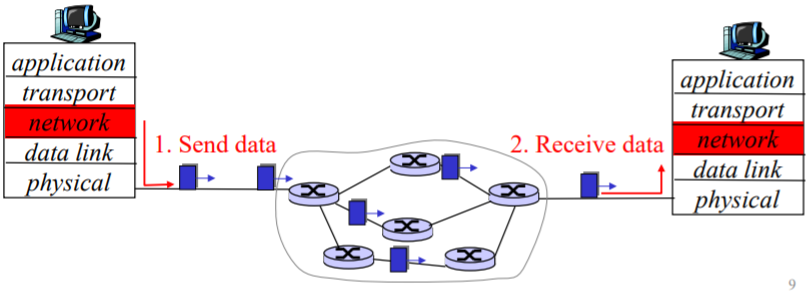
\includegraphics[width=12cm]{images/RCOM2.png}
    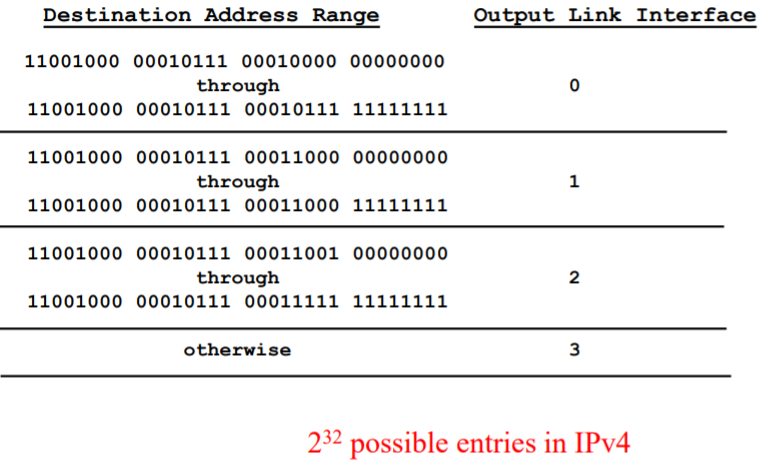
\includegraphics[width=12cm]{images/RCOM3.png}
\end{center}

\subsection{Circuitos Virtuais}
\begin{itemize}
    \item Serviço orientado à ligação
	\item Fases:
	\begin{enumerate}
	    \item Estabelecer o circuito
		\item Transferência de dados
		\item Terminação do circuito
	\end{enumerate}
	\item Cada pacote carrega um identificador do circuito virtual
    \item Caminho da fonte ao destino -> sequência de identificadores virtuais, um para cada ligação
	\item Estado de cada circuito mantido pelo router, que pode alocar recursos (bandwidth, buffers) por circuito virtual
\end{itemize}
\subsubsection{Forwarding Table}
Contém prefixos e a respetiva porta de saída <Endereço/Mask, port>
\begin{center} 
    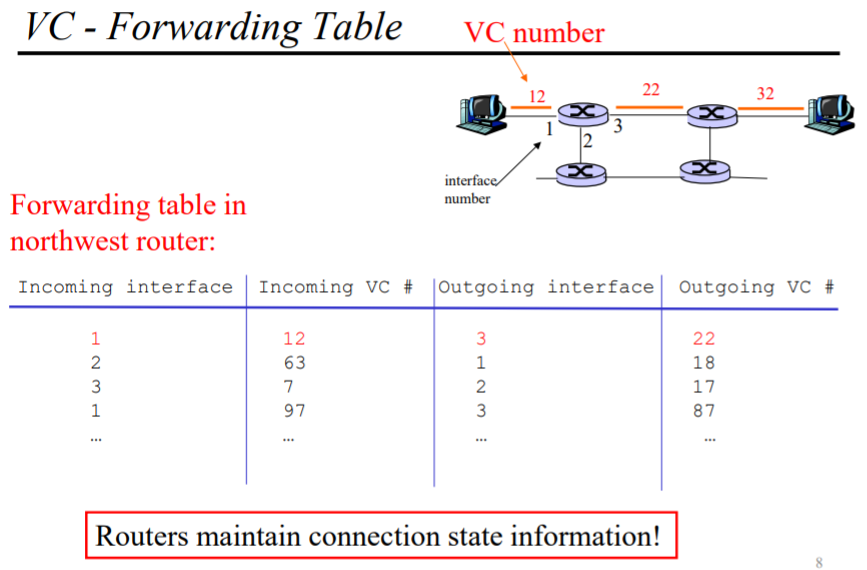
\includegraphics[width=12cm]{images/RCOM1.png}
\end{center}
\subsubsection{Ex: Maior correspondência de prefixo}
\begin{center}            
    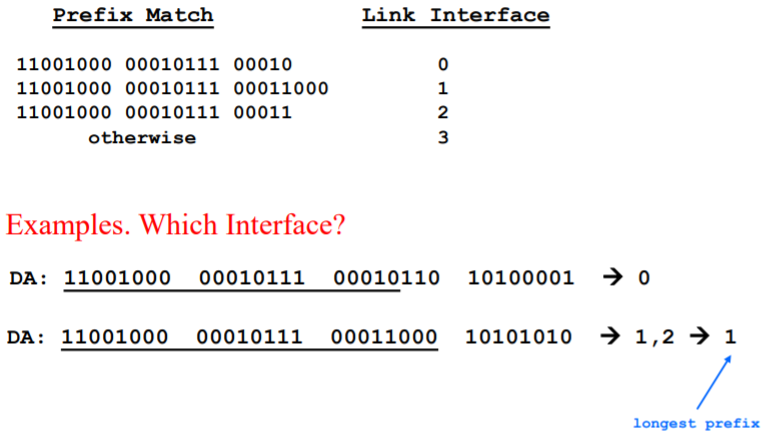
\includegraphics[width=12cm]{images/RCOM4.png}
\end{center}

\subsection{Circuitos Virtuais versus Rede de Datagramas}
\begin{center}            
    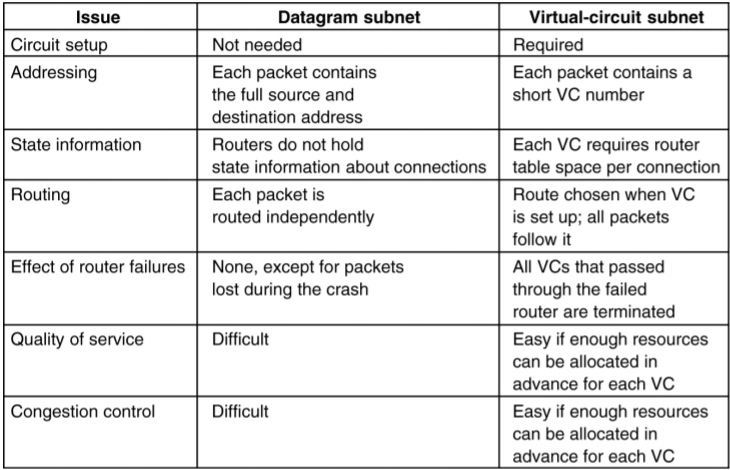
\includegraphics[width=12cm]{images/RCOM5.png}
\end{center}

\subsubsection{Exame 2016 Recurso - Ex:6}
\begin{center}            
    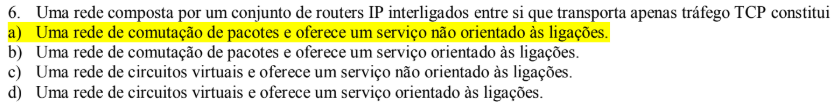
\includegraphics[width=12cm]{images/RCOM48.png}
\end{center}

\subsection{Arquitetura do router}
\begin{itemize}
    \item Funções principais:
    \begin{itemize}
        \item Correr algoritmos de roteamento e protocolos (RIP, OSPF, BGP)
		\item Reencaminhar pacotes
    \end{itemize}
    \item Componentes principais:
    \begin{itemize}
        \item Input Port
        \begin{itemize}
            \item Physical Layer (bit-level)
			\item Data Link Layer (e.g., Ethernet)
			\item Queuing (se os pacotes chegarem rápido demais)
			\item Lookup + Forwarding (faz algum reencaminhamento imediatamente)
        \end{itemize}
        \item Output Port
        \begin{itemize}
            \item Buffering (quando é excedida a velocidade de saída)
			\item Queuing (com disciplina de agendamento)(Queuing perda e espera - devido ao overflow do buffer da porta de input)
			\item Data Link Layer (protocol, desencaplsulação)
			\item Physical Layer (linha de terminação)
        \end{itemize}
        \item Switching Fabric
        \begin{itemize}
            \item Controla o reencaminhamento (fisicamente ou através dum CPU)
            \item Switching Via Memória do Computador
            \begin{itemize}
                \item Router de primeira geração
                \item Em computadores tradicionais, switching é controlado pelo CPU
                \item Cada pacote é copiado para a memória do sistema e transferida duas vezes pelo bus
            \end{itemize}
            \begin{center}
                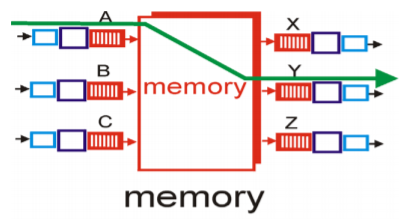
\includegraphics[width=5cm]{images/RCOM6.png}
                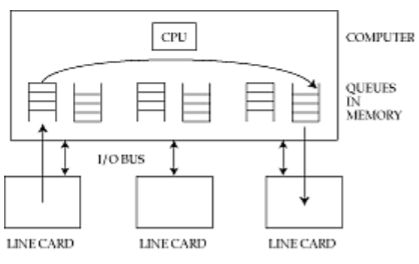
\includegraphics[width=8cm]{images/RCOM9.png}
            \end{center}
            \item Switching via a Bus
            \begin{itemize}
                \item Os pacotes sao processados por um bus partilhado
                \item A transferência dos pacotes desde a linha de input e output é realizada de foram direta
                \item A taxa da conecção do bus é limitada pela bus bandwidth
            \end{itemize}
            \begin{center}
                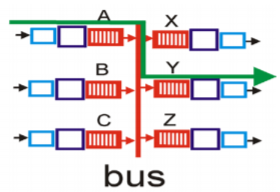
\includegraphics[width=5cm]{images/RCOM7.png}
                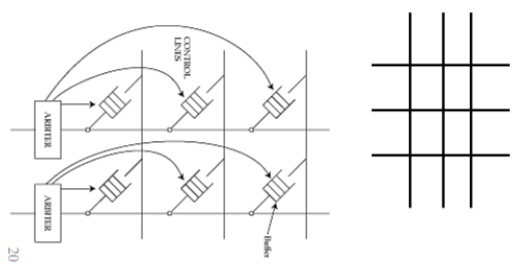
\includegraphics[width=9cm]{images/RCOM10.png}
            \end{center}
            \item Switching via a Crossbar
            \begin{itemize}
                \item 2N buses
                \item Possibilita transferências simultaneas de pacotes
                \item a cross bar pode conter buffers intermos
                \item Ultrapassa os limites da bus bandwidth
            \end{itemize}
            \begin{center}
                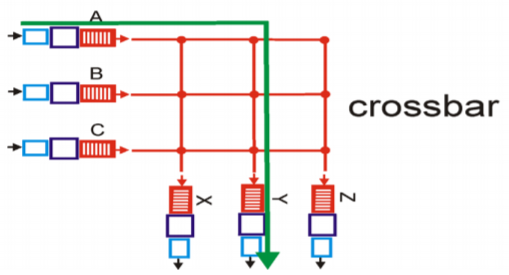
\includegraphics[width=5cm]{images/RCOM8.png}
            \end{center}
        \end{itemize}
        Exame 2016 Normal - Ex.7
        \begin{center}
            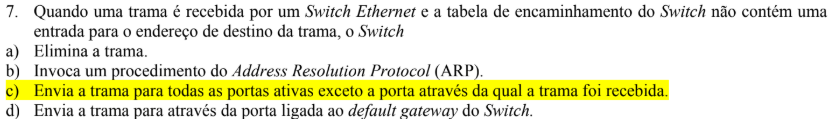
\includegraphics[width=12cm]{images/RCOM51.png}
        \end{center}
    \end{itemize}
\end{itemize}

\subsection{Protocolo Internet}

\begin{enumerate}
    \item Camada de rede Internet
        \begin{center}
            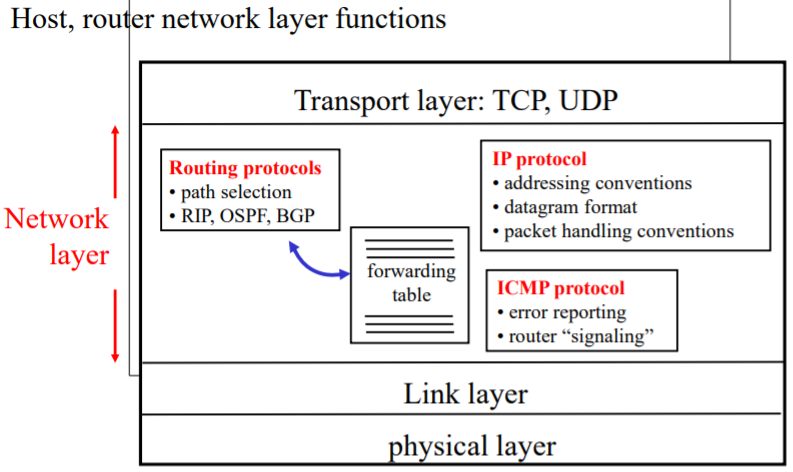
\includegraphics[width=12cm]{images/RCOM11.png}
        \end{center}
    \item Formato datagrama IP
        \begin{center}
            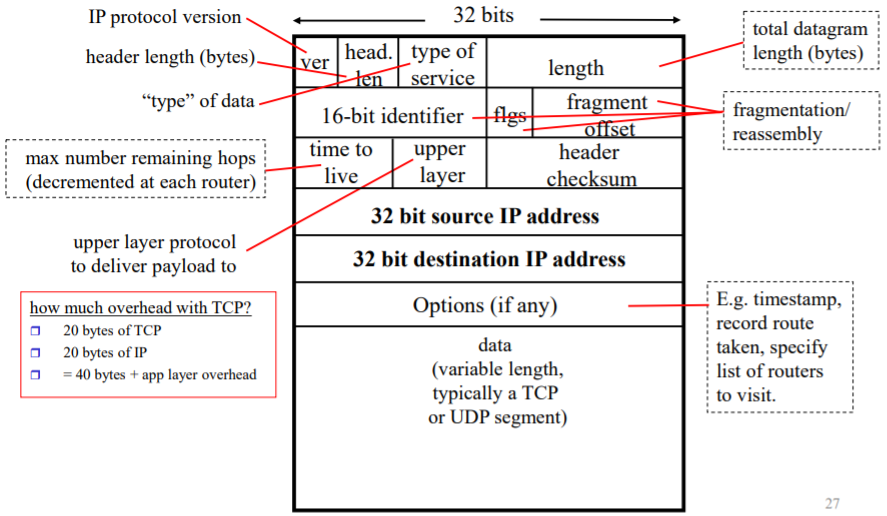
\includegraphics[width=12cm]{images/RCOM12.png}
        \end{center}
    \item Internet Checksum
        \begin{center}
            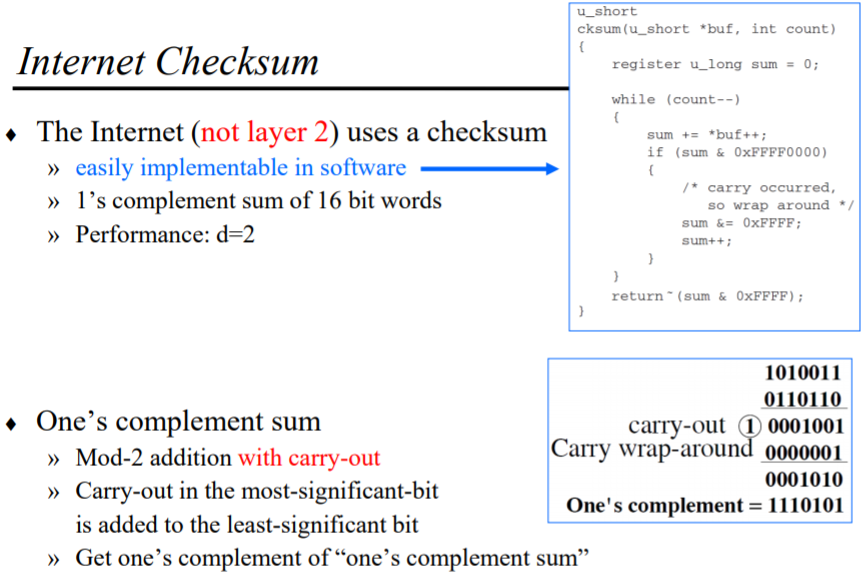
\includegraphics[width=12cm]{images/RCOM13.png}
        \end{center}
\end{enumerate}

\subsubsection{Cada pacote contém:}
\begin{itemize}
    \item Versão do protocolo IP
	\item Tamanho do Header
	\item Tipo de serviço
	\item Tamanho da informação
	\item Identificador + Flags + Offset de Fragmento (Permite fragmentar mensagens em vários pacotes)
	\item Time To Live (para os pacotes não ficarem indefinidamente perdidos na rede)
	\item Upper Layer Protocol
	\item Checksum do Header
	\item IP de Origem
	\item IP de Destino
	\item Opções (opcional)
	\item Informação (Normalmente pacote TCP ou UDP)
\end{itemize}

\subsubsection{Fragmentação IP e Reassembly}
\begin{itemize}
    \item Identificador <- Identifica o pacote
    \item fragflag <- 1 se houver mais informação, 0 se for o último fragmento
	\item Offset <- Offset do fragmento em bytes / 8
\end{itemize}
\begin{center}
    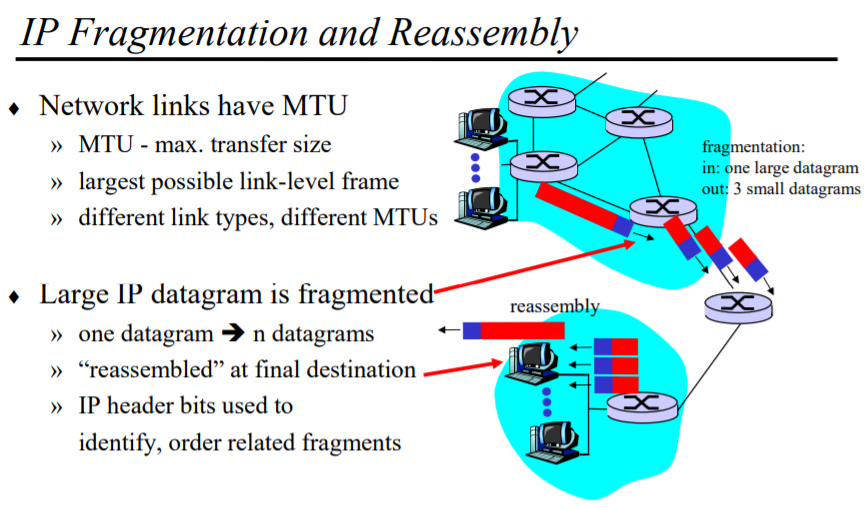
\includegraphics[width=14cm]{images/RCOM14.png}
    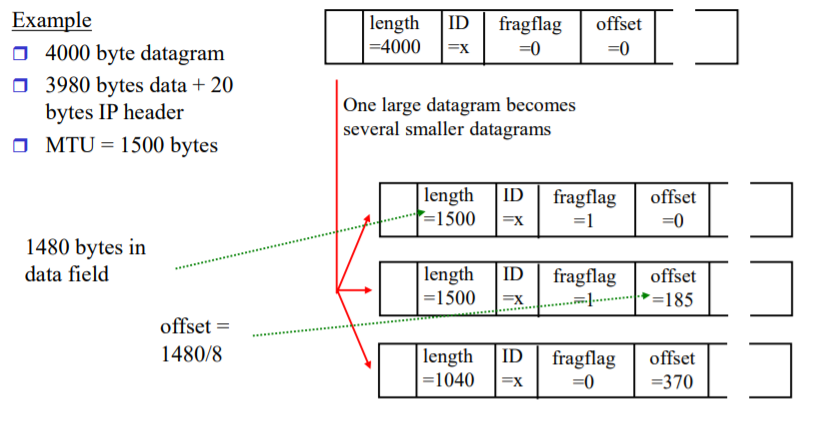
\includegraphics[width=14cm]{images/RCOM15.png}
\end{center}

\subsubsection{Endereço IP}
Endereço IP -  é formado por um identificador de  32-bit para uma interface host/router
Interface possuem:
\begin{itemize}
    \item conecção entre host/router e link físico(physical link)
    \item routers com multiplas interfaces
    \item endereços IP associados com as interfaces
\end{itemize}
\begin{center}
    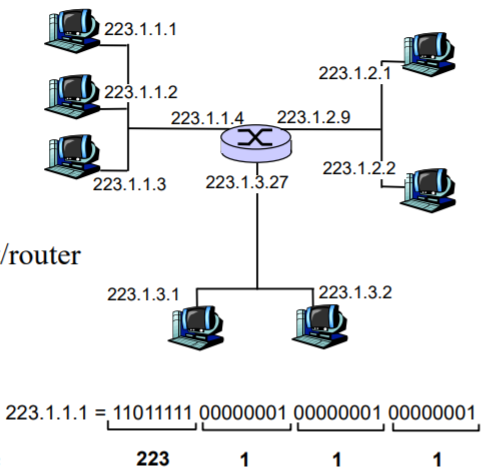
\includegraphics[width=8cm]{images/RCOM16.png}
\end{center}

\subsubsection{Subnets}
\begin{itemize}
    \item Parte mais significativa do IP: Subnet parte
    \item Parte menos significativa: host(interface) parte
	\item Subnet é um set de interfaces
	\item cada um tem a subnet parte do IP igual para comunicação
	\item Cada computador consegue aceder a outro sem intervenção do router
\end{itemize}
\begin{center}
    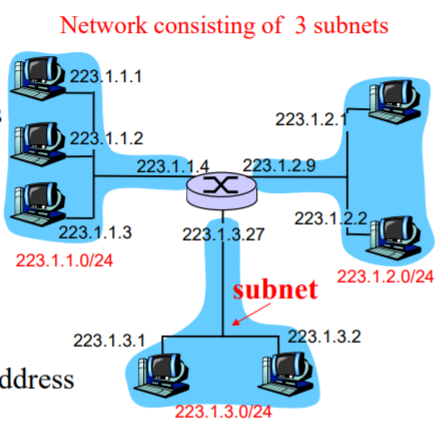
\includegraphics[width=8cm]{images/RCOM17.png}
\end{center}

CIDR - Classless InterDomain Routing
\begin{itemize}
    \item a porção de bits do endereço subnet tem tamanho arbitrário
    \item formato -> a.b.c.d/x, em que x é o número de bits na porção do endereço subnet
\end{itemize}
\begin{center}
    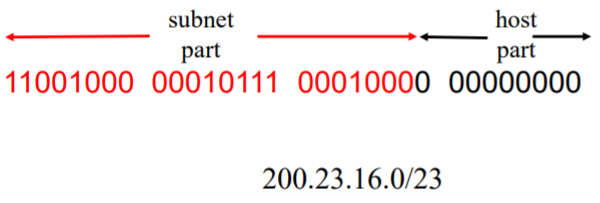
\includegraphics[width=8cm]{images/RCOM18.png}
\end{center}

\subsubsection{Endereços especiais}
\begin{center}
    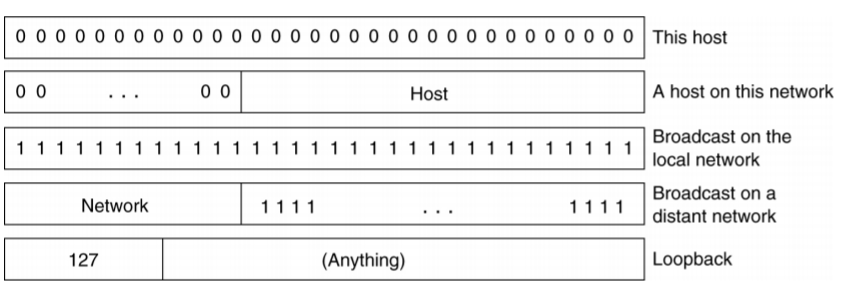
\includegraphics[width=14cm]{images/RCOM19.png}
\end{center}
\begin{itemize}
    \item 0.0.0.0 - este host
    \item 127.0.0.0 - loopback
    \item 255.255.255.255 - broadcast
    \item x.x.255.255 - broadcast na subnet x.x.0.0/16
    \item x.x.0.0 - subnet x.x.0.0/16
\end{itemize}

De Notar: - Uma subrede xx.xx.xx.0/24 suporta 255 endereços, no entanto, dois já estão reservados (xx.xx.xx.0 e xx.xx.xx.255), logo só suporta 253 máquinas.

\textbf{Forming Sub-Networks (importante)}
\begin{center}
    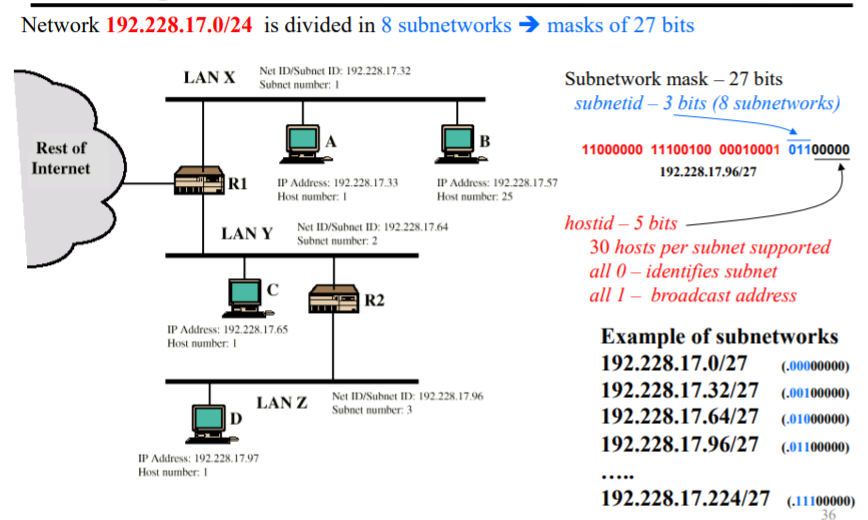
\includegraphics[width=12cm]{images/RCOM20.png}
\end{center}

\textbf{Criar table em R1 (importante)}
\begin{center}
    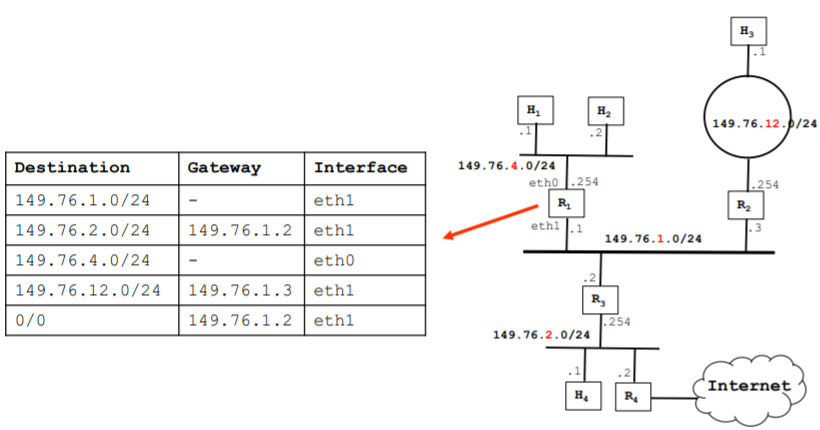
\includegraphics[width=12cm]{images/RCOM21.png}
\end{center}

\textbf{Exercício: Exame 2018R-ultima questao (3)}
Considere que a uma empresa foi atribuído o bloco de endereços IP 20.20.20.128/26. A empresa tem um rede de comunicações com a arquitetura descrita na figura, composta por 4 routers (R1, R2, R3, R4) e 3 switches Ethernet. 
Um dos switches serve 24 computadores, outro serve 13 computadores e o terceiro interliga os routers R1, R2 e R3. Os routers R3 e R4 estão interligados por uma ligação ponto-a-ponto, à qual foi atribuído o endereço de rede 20.20.20.180/30.

\begin{center}
    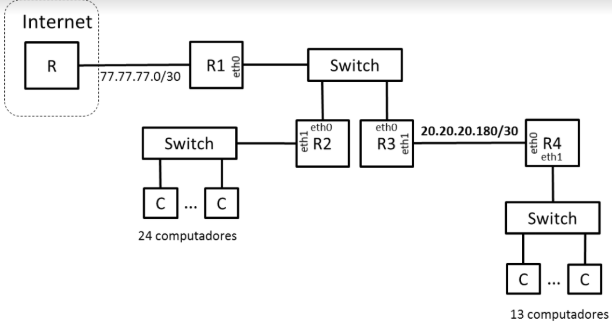
\includegraphics[width=12cm]{images/RCOM40.png}
\end{center}
\textbf{a) Calcule os endereços de rede associados às redes indicadas}
\begin{center}
    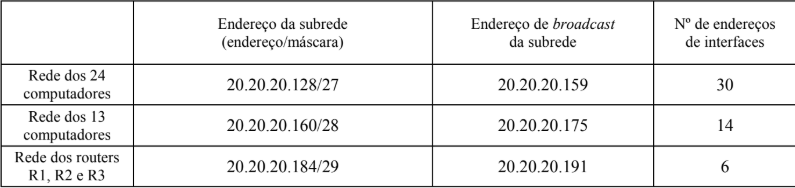
\includegraphics[width=12cm]{images/RCOM41.png}
    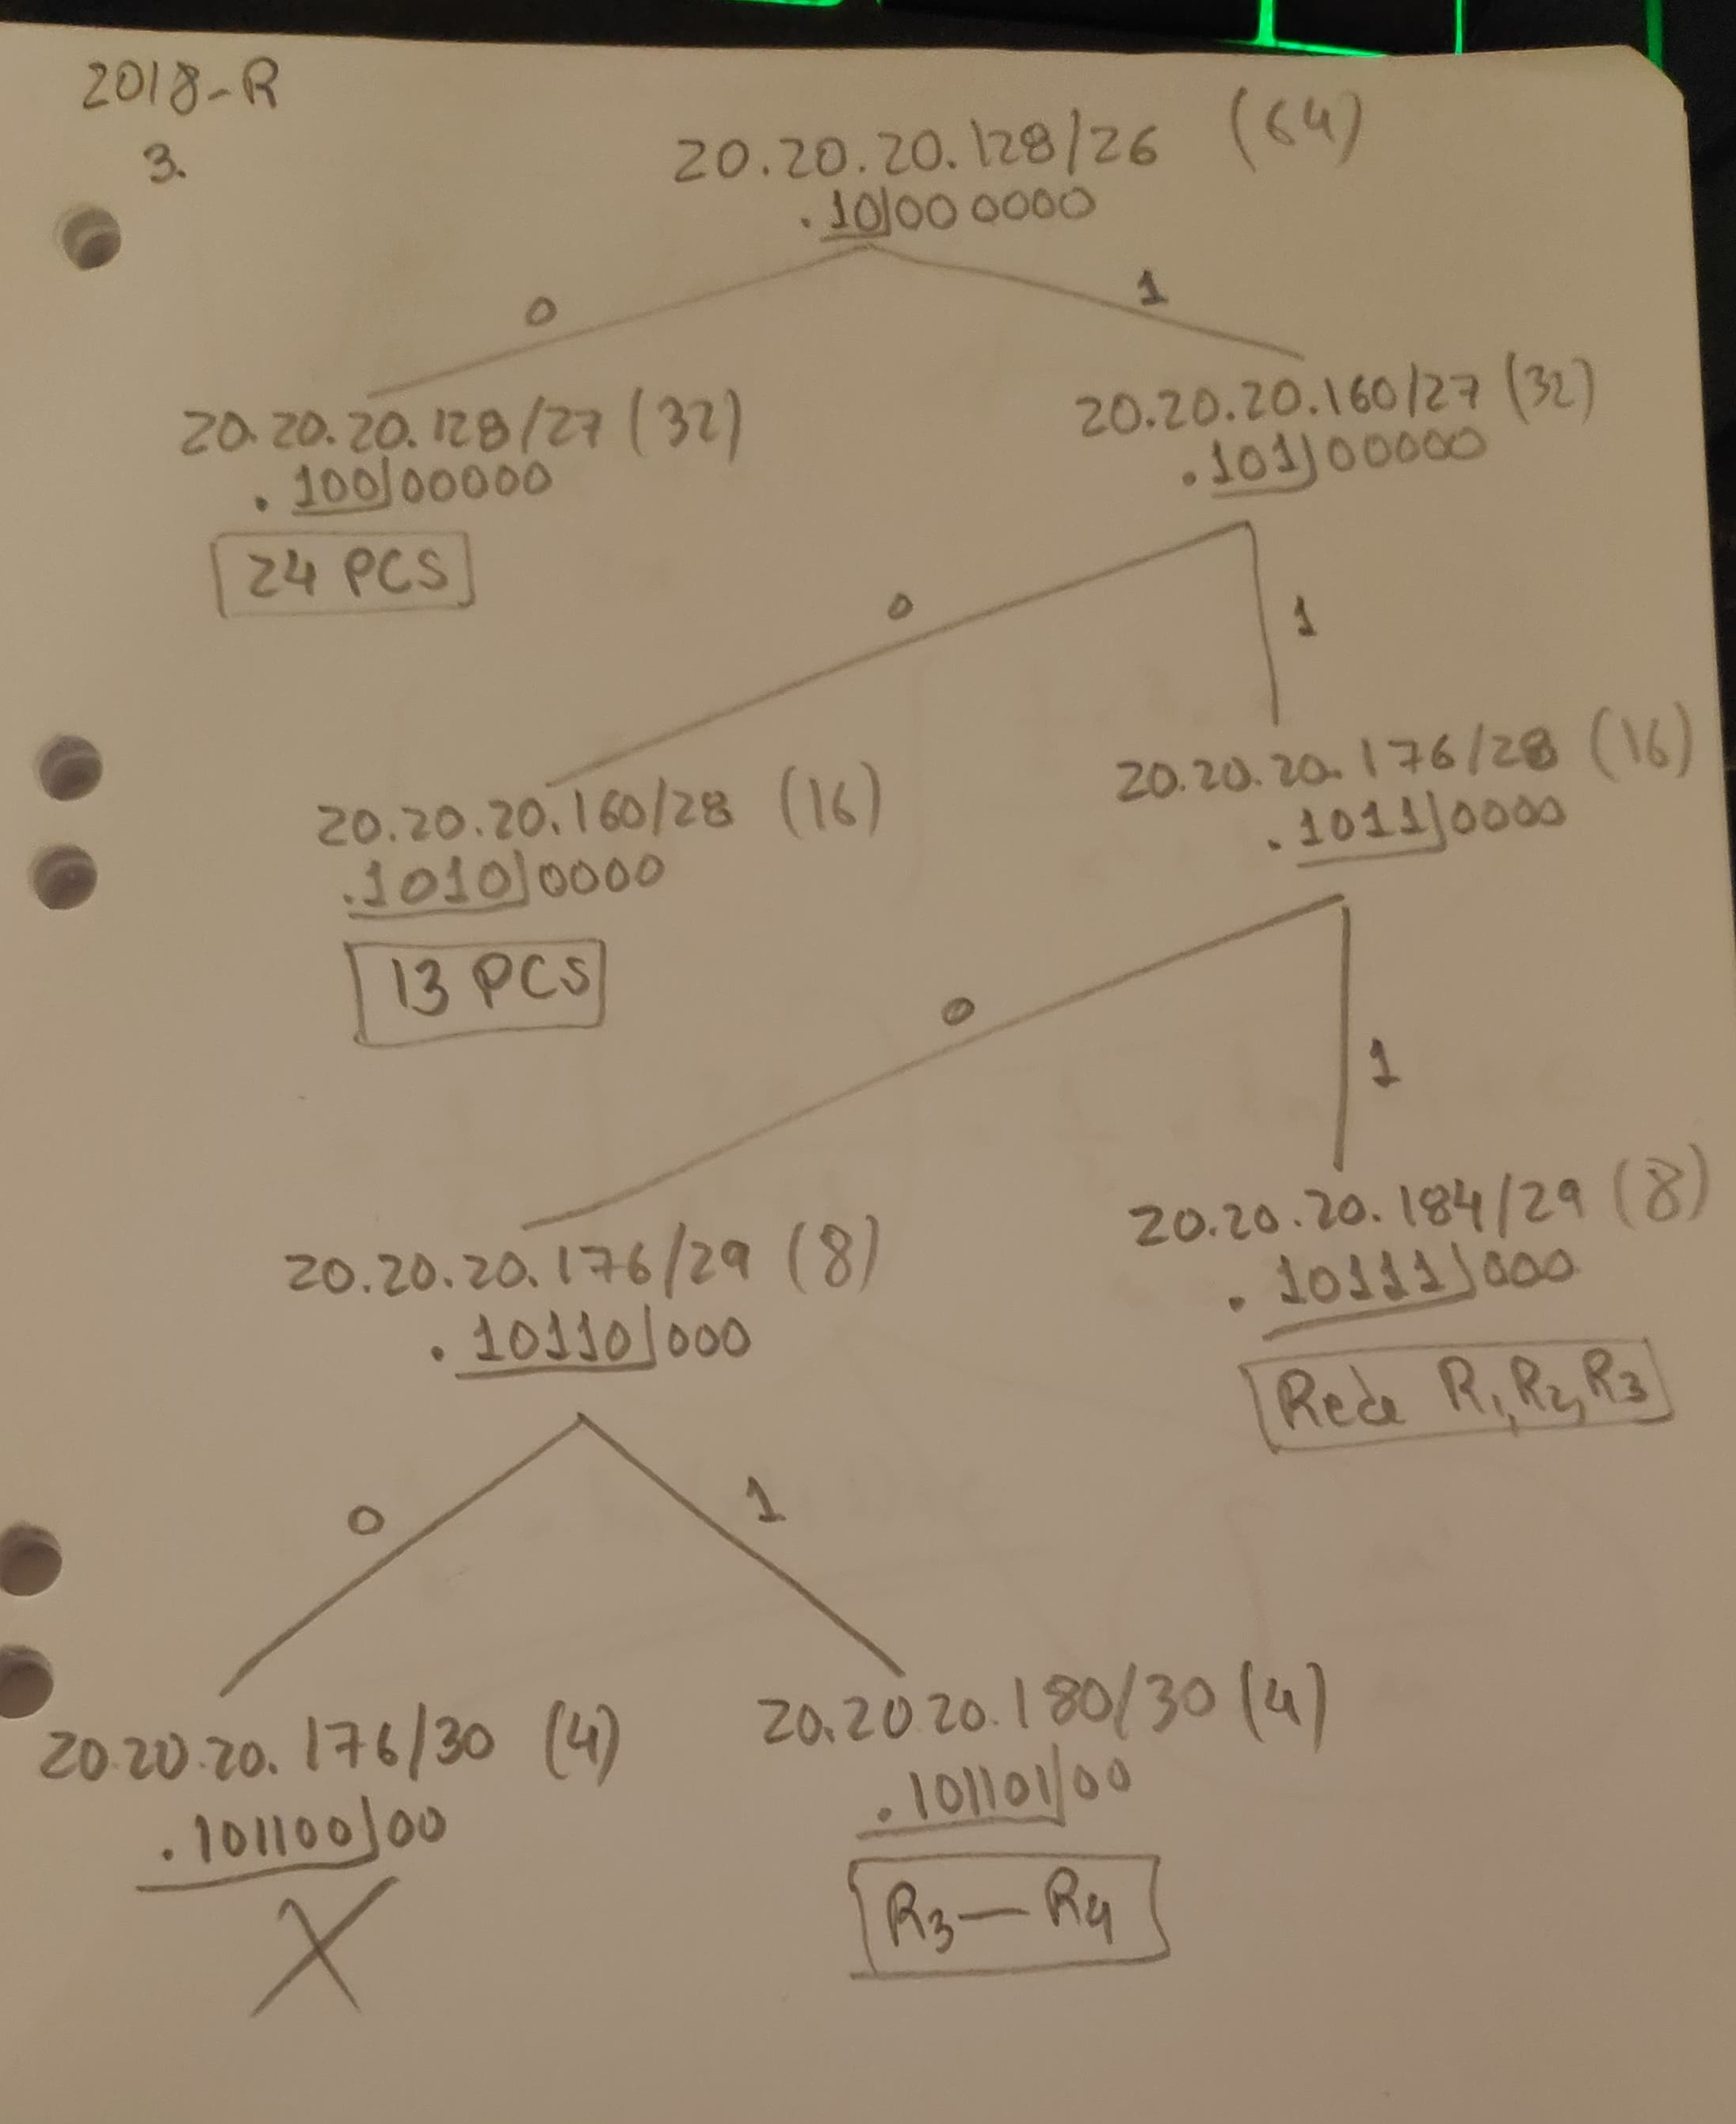
\includegraphics[width=12cm]{images/RCOM55.jpg}
\end{center}
\textbf{b) Atribua endereços IP às interfaces dos routers R1, R2, R3 e R4. Use os endereços mais baixos de cada sub-rede. Numa sub-rede atribua os endereços mais baixos aos routers de índice Ri mais baixo. Por exemplo, o endereço de R3.eth1 deverá ser inferior ao endereço R4.eth0.}
\begin{center}
    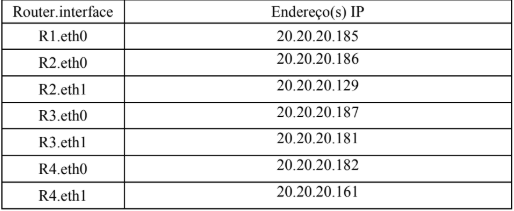
\includegraphics[width=12cm]{images/RCOM42.png}
\end{center}
\textbf{c) Escreva a tabela de encaminhamento do router R2. Este router deverá ser capaz enviar pacotes para todos os endereços IP unicast. Use o menor número possível de entradas na tabela.}
\begin{center}
    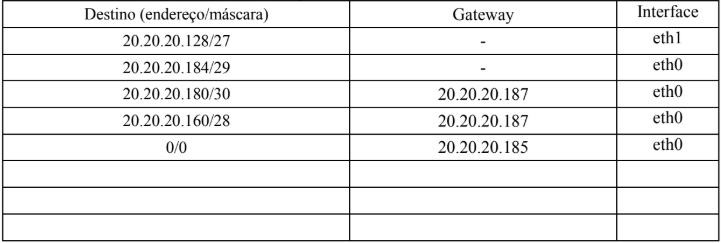
\includegraphics[width=14cm]{images/RCOM43.png}
\end{center}
\textbf{Fazer pergunta 3 (last question) de todos os exames. É igual, apenas alterando os valores dos IPs}

\textbf{função IP forwarding (importante)}
\begin{center}
    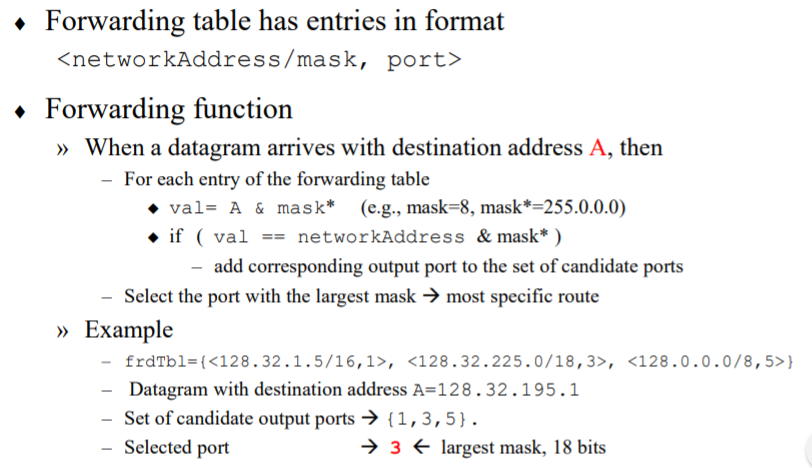
\includegraphics[width=15cm]{images/RCOM22.png}
\end{center}
\textbf{Exame 2018N - Exercicio 7}
\begin{center}
    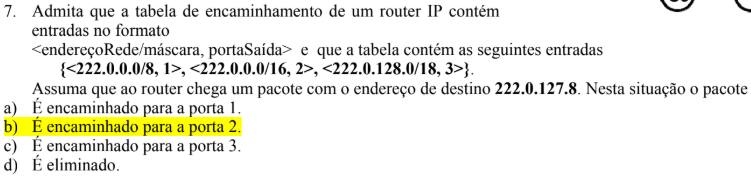
\includegraphics[width=15cm]{images/RCOM45.png}
\end{center}

\subsection{Address Resolution Protocol APR}
\begin{center}
    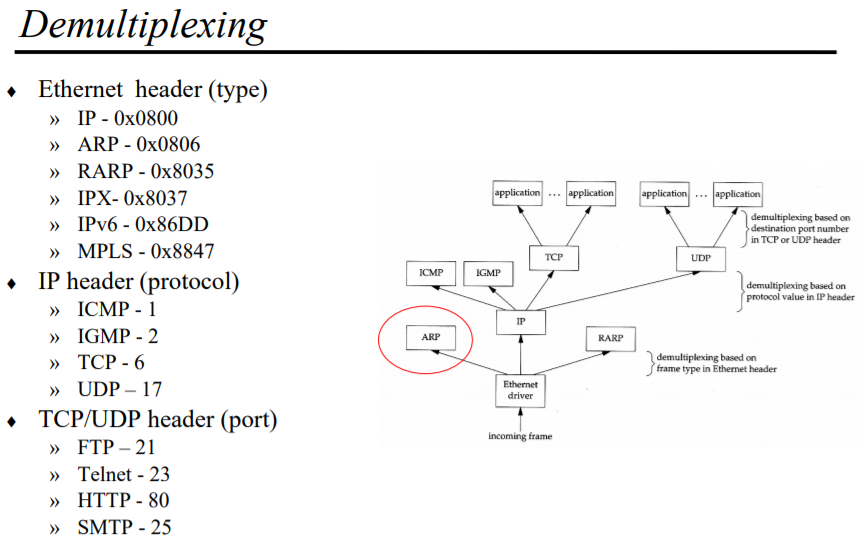
\includegraphics[width=14cm]{images/RCOM23.png}
\end{center}

\begin{itemize}
    \item Uma interface de rede tem 1 endereço MAC e 1 (ou mais) endereços IP
    \item ARP - protocolo usado para obeter o endereço MAC associado a um endereço IP dado
    \item RARP - reverso de ARP - protocolo usado para obter o endereço IP associado ao endereço MAC
\end{itemize}

\begin{center}
    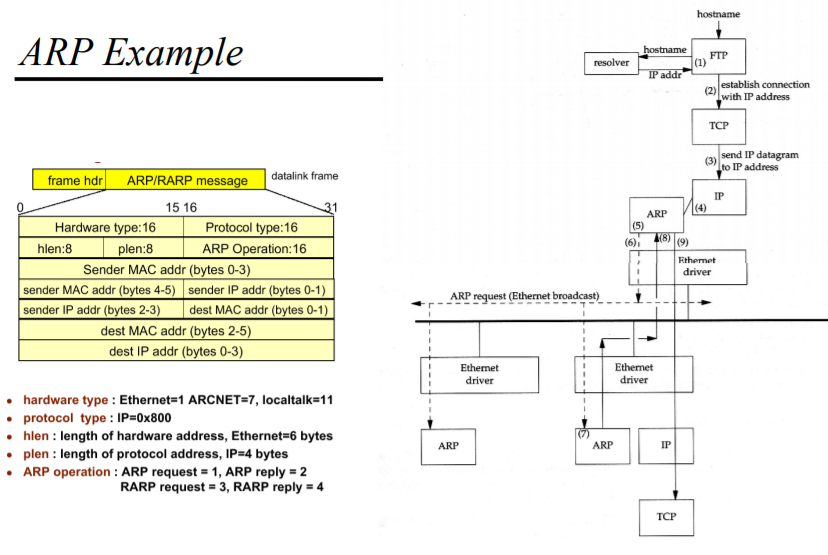
\includegraphics[width=14cm]{images/RCOM24.png}
\end{center}

\subsection{Obter endereço IP}
\begin{itemize}
    \item Parte do endereço da subnet é definido pelo ISP
    \begin{center}
        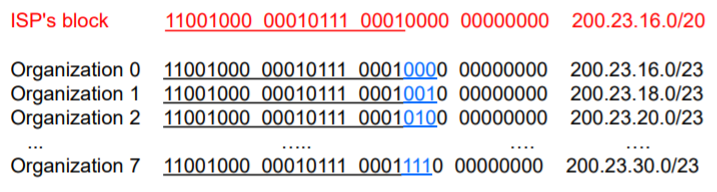
\includegraphics[width=14cm]{images/RCOM25.png}
    \end{center}
    \item endereçamento hierárquico permite eficiência da informação do router
    \item O ISP depois trata internamente das suas subredes
    \item O ISP obtém endereços pela ICANN
    \item ICANN: Internet Corporation for Assigned Names and Numbers
    \begin{itemize}
        \item aloca endereços
        \item controla o Domain Name Service (DNS)
        \item associa os nomes do domínio
        \item resolve conflitos
    \end{itemize}
    \item o host obtém endereços IP de forma hard-coded pelo sistema admin num ficheiro ou pelo DHCP
    \item DHCP: Dynamic Host Configuration Protocol
    \begin{itemize}
        \item Dinamicamente recebe endereços do servidor
        \item "plug-and-play"
        \item permite descobrir e obter endereços da rede do servidor
        \item reusa os endereços
        \item Overview:
        \begin{itemize}
            \item O host faz broadcast de "DHCP discover" (msg)
            \item O servidor DHCP oferece um endereço, enviando em broadcast "DHCP offer" (msg)
			\item O host pede esse endereço enviando em broadcast "DHCP request" (msg)
            \item Se tudo estiver em ordem, o DHCP responde em broadcast com um "DHCP ACK" (msg)
            \item Todas as mensagens entre o host e o DHCP possuem um id de transação
        \end{itemize}
    \end{itemize}
\end{itemize}

(Com o seguinte gráfico analisar pergunta 7 do exame 2018N)
\begin{center}
    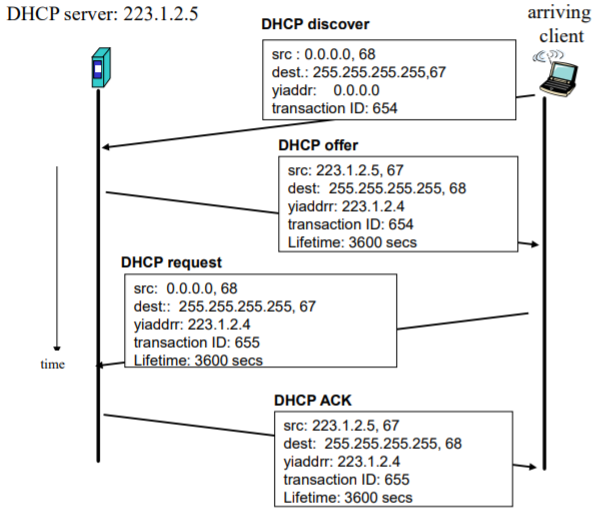
\includegraphics[width=12cm]{images/RCOM26.png}
\end{center}

\subsection{NAT - Network Address Translation}
\begin{itemize}
    \item Permite que cada computador tenha um IP interno numa rede, sendo o IP externo diferente
    \item Para isso, possui uma hash table a que associa um IP interno e uma porta a um número, que será a porta de saída
    \item Caso um cliente se queira ligar a um servidor dentro de uma rede com NAT, é necessário configurar o port forwarding

\end{itemize}
\begin{center}
    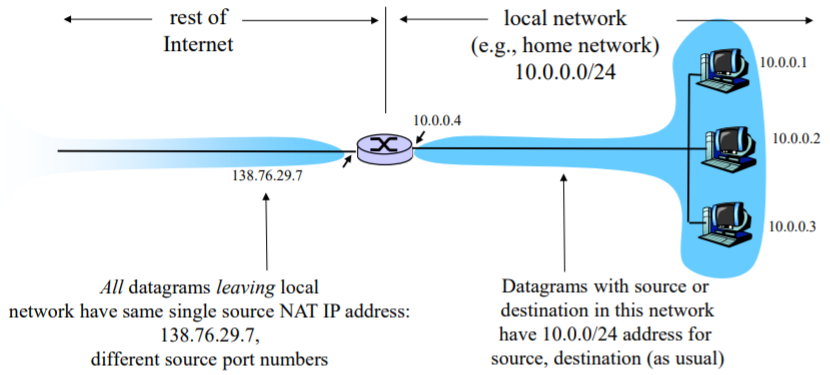
\includegraphics[width=10cm]{images/RCOM27.png}
    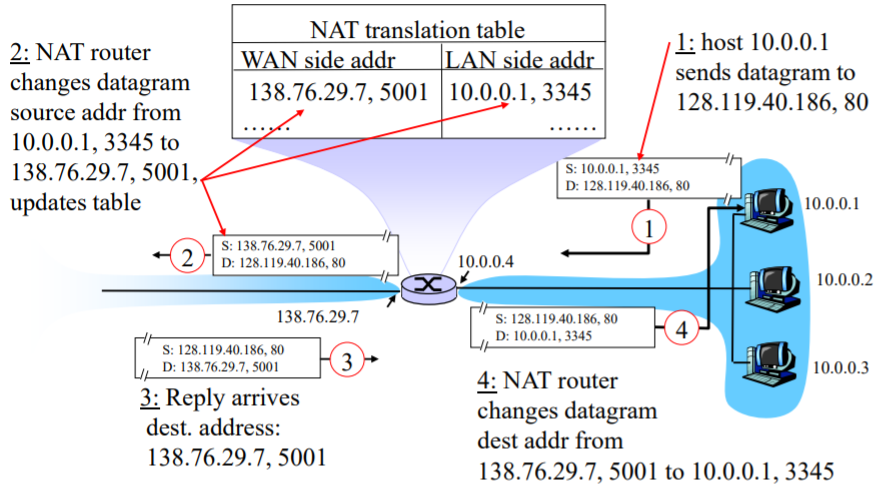
\includegraphics[width=10cm]{images/RCOM28.png}
\end{center}

\subsubsection{NAT Transversal}
\begin{center}
    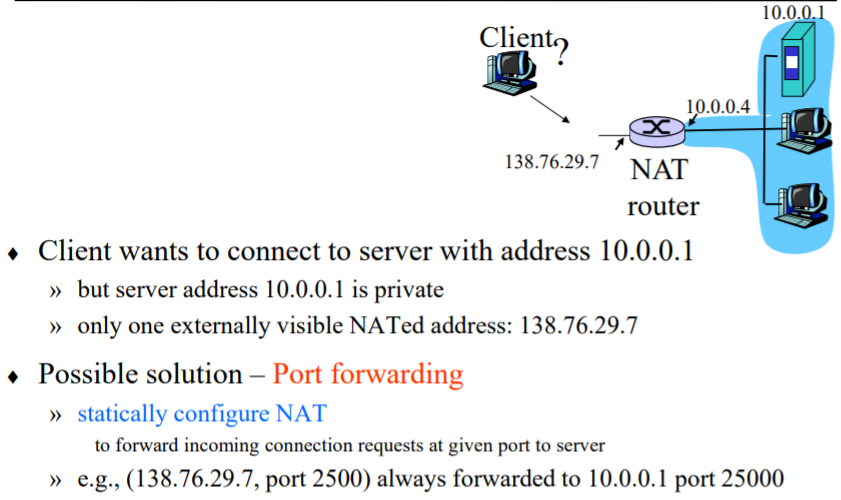
\includegraphics[width=12cm]{images/RCOM29.png}
\end{center}

\subsubsection{Question 8 - Exame 2017N}
\begin{center}
    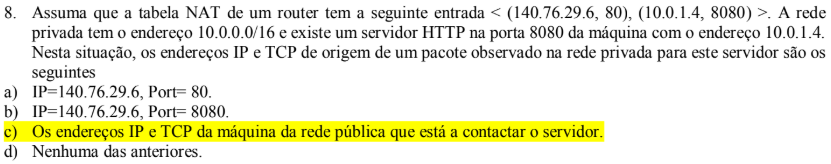
\includegraphics[width=12cm]{images/RCOM47.png}
\end{center}

\subsection{ICMP - Internet Message Control Protocol}

- Usado pelo router ou host para mandar mensagens de erro ou de controlo (como o ping)

\subsubsection{Exame 2017N Ex:1}
\begin{center}
    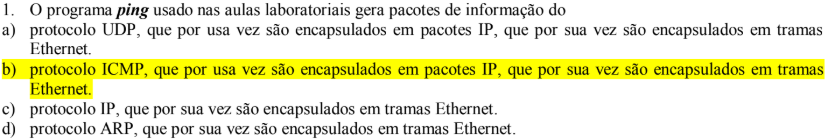
\includegraphics[width=12cm]{images/RCOM46.png}
\end{center}

\subsubsection{Exame 2018N Ex:2}
\begin{center}
    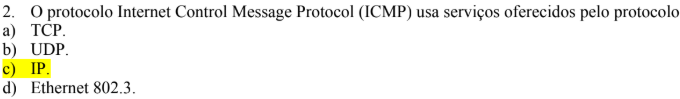
\includegraphics[width=12cm]{images/RCOM44.png}
\end{center}

\subsubsection{Exame 2016 Recurso - Ex:7}
\begin{center}            
    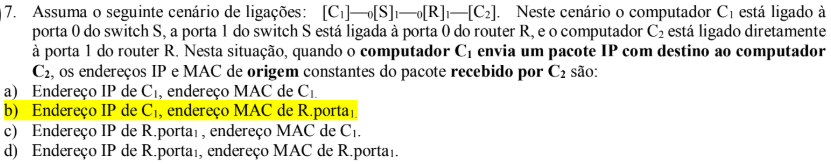
\includegraphics[width=12cm]{images/RCOM50.png}
\end{center}
\subsubsection{Exame 2013 Recurso - Ex:7}
\begin{center}            
    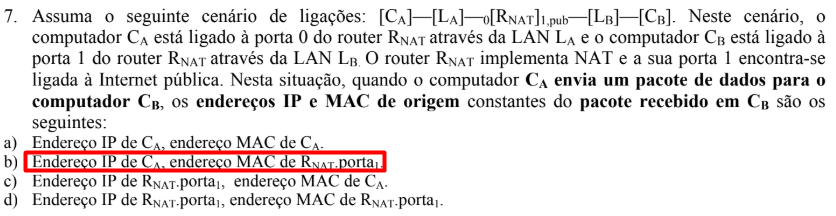
\includegraphics[width=14cm]{images/RCOM53.png}
\end{center}

\subsubsection{Exame 2018 Recurso }
se o computador do segmento C fizer ping ao Computador 
do segmento A, indique os endereços IP e MAC constantes 
do pacote que transporta a mensagem ICMP Echo Request no 
segmento A. (Questão 2018R-ex:9).
\begin{center}
    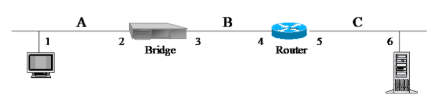
\includegraphics[width=15cm]{images/RCOM49.png}
\end{center}
R: IP origem = 6, IP destino = 1, MAC origem = 4, MAC destino = 1.\newline
\subsubsection{Exame 2014 Normal - Ex:9)}
\begin{center}
    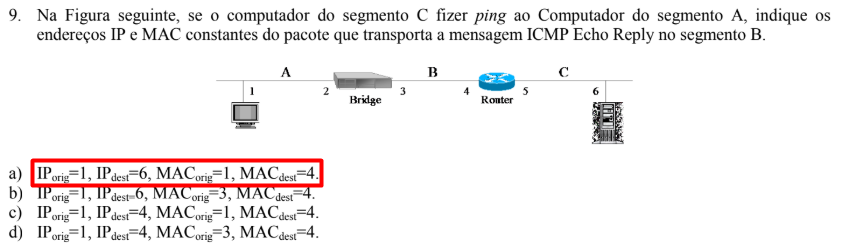
\includegraphics[width=15cm]{images/RCOM52.png}
\end{center}

\subsubsection{Exame 2010 Normal - Ex:4 e 5)}
\begin{center}
    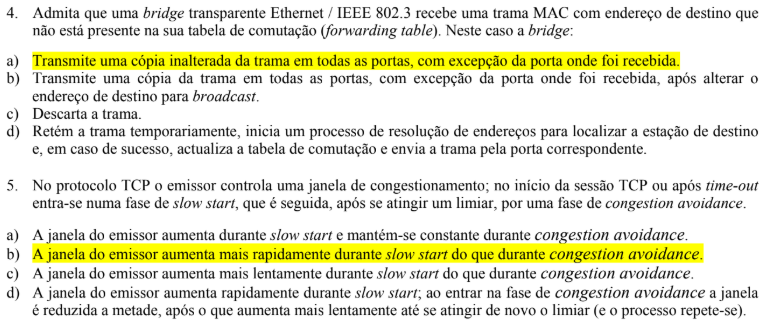
\includegraphics[width=15cm]{images/RCOM54.png}
\end{center}


\subsubsection{IP datagramas info:}
\begin{center}
    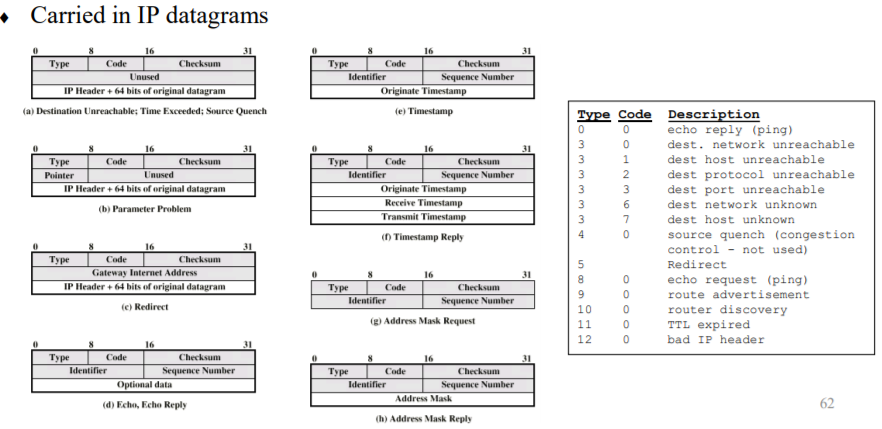
\includegraphics[width=15cm]{images/RCOM30.png}
\end{center}

\subsubsection{Tracerout and ICMP}
- Permite fazer traceroute enviando mensagens com TTL=1,2,3... e esperando respostas de erro	"TTL expired" até receber um "Host unreachable"
\begin{center}
    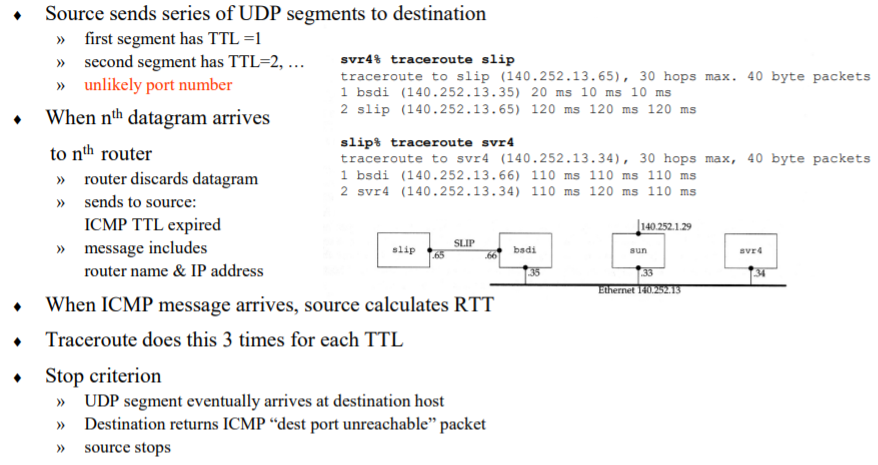
\includegraphics[width=14cm]{images/RCOM31.png}
\end{center}

\subsubsection{ICMP Redirect}
- ICMP Redirect - Permite informar outros hosts do caminho mais rápido para determinado destino

\begin{center}
    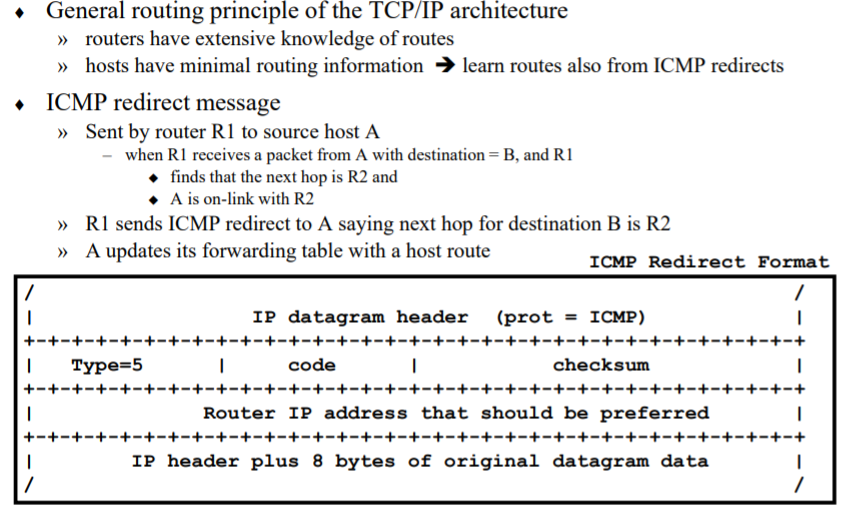
\includegraphics[width=14cm]{images/RCOM32.png}
    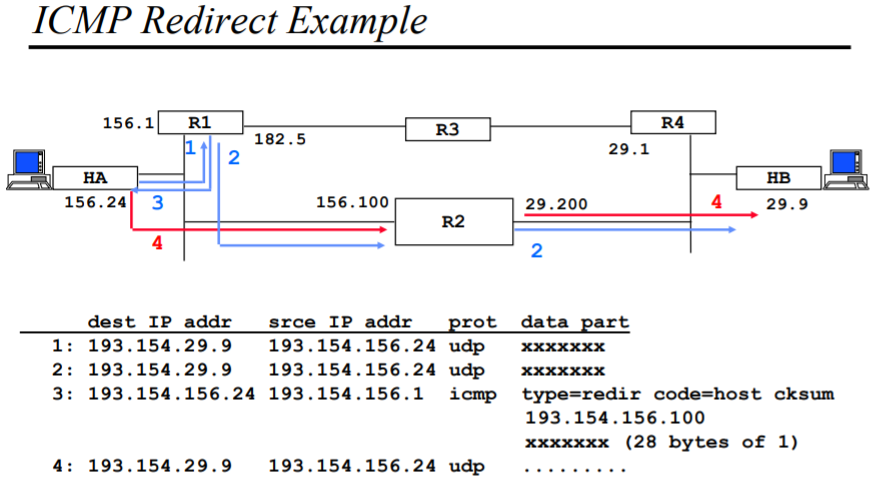
\includegraphics[width=14cm]{images/RCOM33.png}
    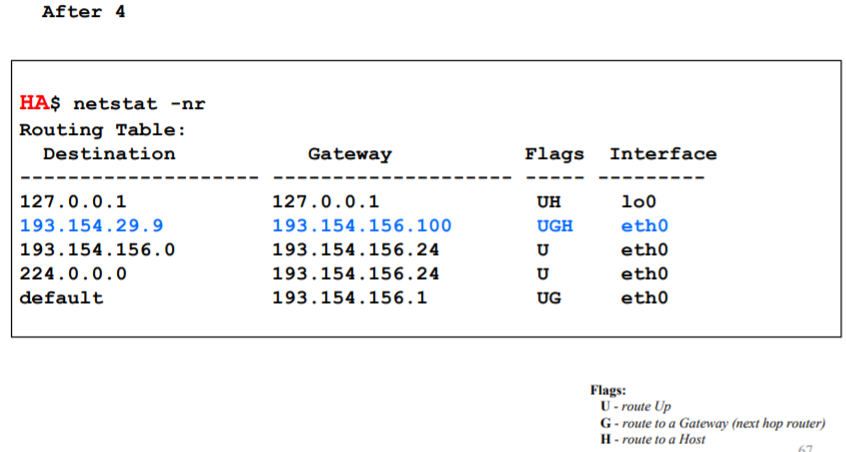
\includegraphics[width=14cm]{images/RCOM34.png}
\end{center}

\subsection{IPv6}
\begin{itemize}
    \item IPv4
    \begin{itemize}
        \item espaço reduzido de endereçamento (32 bits)
        \item uso não continuo
        \item o uso de algumas soluções como private networks (NAT) e classless networks (CDIR) superava os problemas acima
    \end{itemize}
    \item IETF developed new IP version: IPv6
    \begin{itemize}
        \item Uso dos mesmos princípios do IPv4
        \item muitas melhorias
        \item Header foi redefinido
    \end{itemize}
\end{itemize}

\subsubsection{IPv6 - Melhorias}
\begin{itemize}
    \item Endereços 128 bits (16 octets, 8 shorts). No classes
    \item Melhor QoS suporte (native flow level)
    \item funções nativas de segurança (autenticação, data encriptação)
    \item Autoconfiguração (Plug-n-play)
    \item Routing
    \item Multicast
\end{itemize}

\subsubsection{Representação dos endereços}
\begin{itemize}
    \item 8 x 16 bit, hexadecimal, separados por:\newline \textbf{47CD : 1234 : 3200 : 0000 : 0000 : 4325 : B792 : 0428}
    \item formato comprimido:\newline \textbf{FF01:0:0:0:0:0:0:43 -> FF01::43}
    \item compatibilidade com IPv4:\newline \textbf{0:0:0:0:0:0:13.1.68.3 or ::13.1.68.3}
    \item Loopback endereço:\newline \textbf{::1}
    \item Prefixo de rede "/", igual ao IPv4:\newline \textbf{FEDC:BA98:7600::/40 -> network prefix = 40 bits}
\end{itemize}

\subsubsection{Endereços Reservados}
\begin{center}
    \includegraphics[width=12cm]{images/RCOM35.png}
\end{center}

\subsubsection{Tipo de Endereços}
\begin{itemize}
    \item Link-Local
    \begin{itemize}
        \item Usado para a comunicação entre hosts na mesma LAN/link
        \item Endereço criado pelo endereço MAC
        \item Routers nao enviam pacotes tendo endereços de destino Link-Local
    \end{itemize}
    \item Global Unicast
    \begin{itemize}
        \item Endereços globais
        \item Endereços: prefixo de rede + identificador do computador
        \item Prefixos estruturados: Agregação de rede; menos entradas nas router forwarding tables
    \end{itemize}
    \item Anycast
    \begin{itemize}
        \item Endereços de grupo
        \item Um pacote é recebido por um e um só membro do grupo
    \end{itemize}
    \item Multicast
    \begin{itemize}
        \item Endereços de grupo
        \item Um pacote pode ser recebido por vários membros do grupo
    \end{itemize}
\end{itemize}

\subsubsection{Formato dos Endereços}
\begin{center}
    \includegraphics[width=15cm]{images/RCOM36.png}
\end{center}

\subsubsection{Headers IPv4 e IPv6}
\begin{center}
    \includegraphics[width=14cm]{images/RCOM37.png}
\end{center}

\subsubsection{IPv6 Header}
\begin{itemize}
    \item Flow label - identifica o fluxo do pacote
    \begin{itemize}
        \item QoS, ressalva de recursos
        \item Pacotes recebem o mesmo serviço
    \end{itemize}
    \item Payload lenght - Header não incluído
    \item Next header - identifica o próximo header/extensão
    \item Options - incluída nas extensões dos headers
\end{itemize}

\subsubsection{Extension Headers}
\begin{center}
    \includegraphics[width=14cm]{images/RCOM38.png}
\end{center}
\begin{itemize}
    \item Hop-by-Hop: inspeciona todos os nodes atravessados pelo pacote
    \item Destination: informação do node de destino
    \item Routing: Lista dos nodes para serem visitados pelo pacote
    \item Fragmentation: feito pelo source, deve encontrar MPU
    \item Authentication: autenticação (assinatura) do header do pacote
    \item ESP: encriptação da informação(data)
\end{itemize}

\subsubsection{Exemplo da Rede do Laboratório}
\begin{center}
    \includegraphics[width=14cm]{images/RCOM39.png}
\end{center}

\subsubsection{Protocol Neighbor Discovery (ND)}
IPv6 node usa ND para: 
\begin{itemize}
    \item Encontrar outros nodes no mesmo link/LAN
    \item Encontrar o node do endereço MAC (ND substitui ARP)
    \item Encontrar routers na sua rede
    \item Manter/Segurar a informação sobre os nodes vizinhos
\end{itemize}

ND similar às funções IPv4:
\begin{itemize}
    \item ARP IPv4
    \item ICMP Router Discovery
    \item ICMP Redirect
\end{itemize}

\subsubsection{ND Mensagens}
\begin{itemize}
    \item ICMP mensagens (over IP), Uso de endereços Link Local
    \item \textbf{Neighbor Solicitation: } Enviado pelo host para obter o endereço MAC de um vizinho/para verificar a sua presença
    \item \textbf{Neighbor Advertisement: } resposta ao pedido
    \item \textbf{Router Advertisement: } Informação sobre o prefixo da rede, periodica ou abaixo do pedido. Enviado pelo router para o endereço IP do Link Local multicast
    \item \textbf{Router Solicitation: } Hosts solicitam do router uma mensagem Router Advertisment
    \item \textbf{Redirect: } Usado pelo router para informar o host acerca da melhor rota para o destino
\end{itemize}

\end{document}